
\begin{figure}[H]
\begin{center}
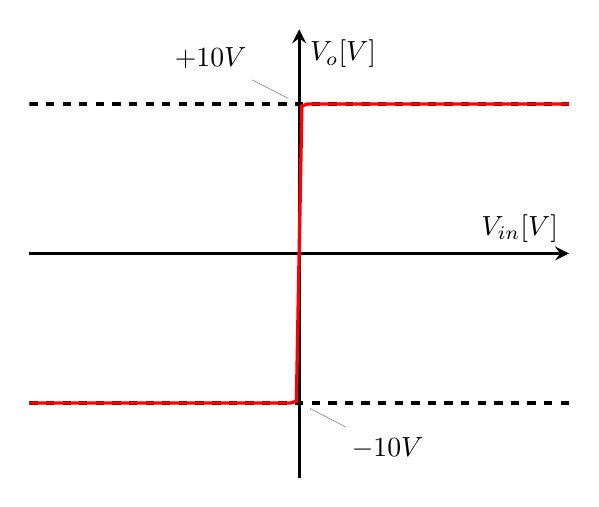
\begin{tikzpicture} 
\begin{axis}[very thick,
                     samples = 100,
                     ytick={-10,10},
                     xlabel = {$V_{in}[V]$},
                     ylabel = {$V_{o}[V]$},
                     xmin = -5,
                     xmax = 5,
                     ymin = -15,
                     ymax = 15,
                     axis x line = middle,
                     axis y line = middle,
                     ticks = none]
            \addplot[dashed] plot (\x, 10);
            \addplot[dashed] plot (\x,-10);
            \addplot[red] plot (\x, {-10+20/(1 + exp(-\x*100))});
            \addplot[mark=none] coordinates {(0,10)} node[pin=150:{$+10V$}]{};
            \addplot[mark=none] coordinates {(0,-10)} node[pin=-30:{$-10V$}]{};
        \end{axis}
\end{tikzpicture}
\end{center}
\caption{Característica de transferência para o comparador não inversor simples.}
\label{graph:1} 
\end{figure}